% Created 2025-11-29 Sat 14:01
% Intended LaTeX compiler: pdflatex
\documentclass[presentation, aspectratio=169, 14pt]{beamer}
\usepackage[utf8]{inputenc}
\usepackage[T1]{fontenc}
\usepackage{graphicx}
\usepackage{longtable}
\usepackage{wrapfig}
\usepackage{rotating}
\usepackage[normalem]{ulem}
\usepackage{amsmath}
\usepackage{amssymb}
\usepackage{capt-of}
\usepackage{hyperref}
\usepackage{booktabs}
\usepackage{tgheros}
\definecolor{mywhite}{HTML}{FFFFFF}
\definecolor{myblack}{HTML}{333333}
\definecolor{slidetitlecolor}{HTML}{FF2233}
\definecolor{mblack}{HTML}{000000}
\definecolor{mybold}{HTML}{000000}
\definecolor{titlecolor}{HTML}{222222}
\definecolor{namecolor}{HTML}{555555}
\usepackage[absolute,overlay]{textpos}
\usepackage{graphicx}
\usepackage{tikz}
\definecolor{R}{HTML}{FF0000}
\usetheme{metropolis}
\author{Rayan Raddatz de Matos}
\date{14/10/2025}
\title{}
\setbeamercolor{background canvas}{bg=mywhite}
\setbeamercolor{frametitle}{fg=mywhite, bg=slidetitlecolor}
\setbeamerfont{frametitle}{size=\small}
\setbeamercolor{alerted text}{fg=mybold}
\setbeamerfont{alerted text}{series=\bfseries}
\setbeamertemplate{section page}{%
\usebeamerfont{section title}\insertsectionhead% Display the section title
\vskip1cm% Add some space below the title
\usebeamerfont{subsection title}\insertsubsectionhead% Display the subsection title (if any)
}
\hypersetup{
 pdfauthor={Rayan Raddatz de Matos},
 pdftitle={},
 pdfkeywords={},
 pdfsubject={},
 pdfcreator={Emacs 28.2 (Org mode 9.5.5)},
 pdflang={Brazilian}}
\begin{document}

\begin{frame}[plain] % O [plain] remove todos os elementos do frame
    % Set the grid for textpos. The {1cm}{1cm} means our coordinates are in cm.
    \setlength{\TPHorizModule}{1cm}
    \setlength{\TPVertModule}{1cm}

    % The textblock environment places the content.
    % Format is: {width of block}(x-position, y-position from top-left corner)
    \begin{textblock*}{2.5cm}(13.2cm, 7cm)
        \includegraphics[width=2.5cm]{~/logos/INF.png}
    \end{textblock*}

    \begin{textblock*}{2.5cm}(.5cm, 6.8cm)
        \includegraphics[width=2cm]{~/logos/UFRGS.png}
    \end{textblock*}

  \begin{center}
      \vspace*{2cm}
      { \color{titlecolor} \textbf{Intrusiveness and Scalability of OMPT-Based Tracing Tools for Task-based OpenMP Applications}}\\[10px]
      {\footnotesize \color{namecolor} \textbf{Rayan Raddatz de Matos}, Lucas Mello Schnorr}\\
      {\tiny \{rayan.raddatz@inf.ufrgs.br, schnorr@inf.ufrgs.br\}}\\[2cm]
      {\footnotesize SSCAD -- Bonito, MS -- October, 2025}
  \end{center}

\end{frame}

\begin{frame}[label={sec:org590cd76}]{Agenda}
\vfill
\begin{itemize}
\item Task-based OpenMP Applications
\end{itemize}
\vfill
\begin{itemize}
\item OMPT-Based Tracing Tools
\end{itemize}
\vfill
\begin{itemize}
\item Intrusiveness and Scalability
\end{itemize}
\vfill
\end{frame}
\section{\small Intrusiveness and Scalability of OMPT-Based Tracing Tools for Task-based OpenMP Applications}
\label{sec:org59c24d7}
\section{\small \color{mblack} Intrusiveness and Scalability of OMPT-Based Tracing Tools for \color{R} Task-based OpenMP Applications}
\label{sec:orged515a1}
\begin{frame}[label={sec:org711bb92}]{Task-based parallelism}
\begin{columns}
\begin{column}{0.5\columnwidth}
\begin{center}
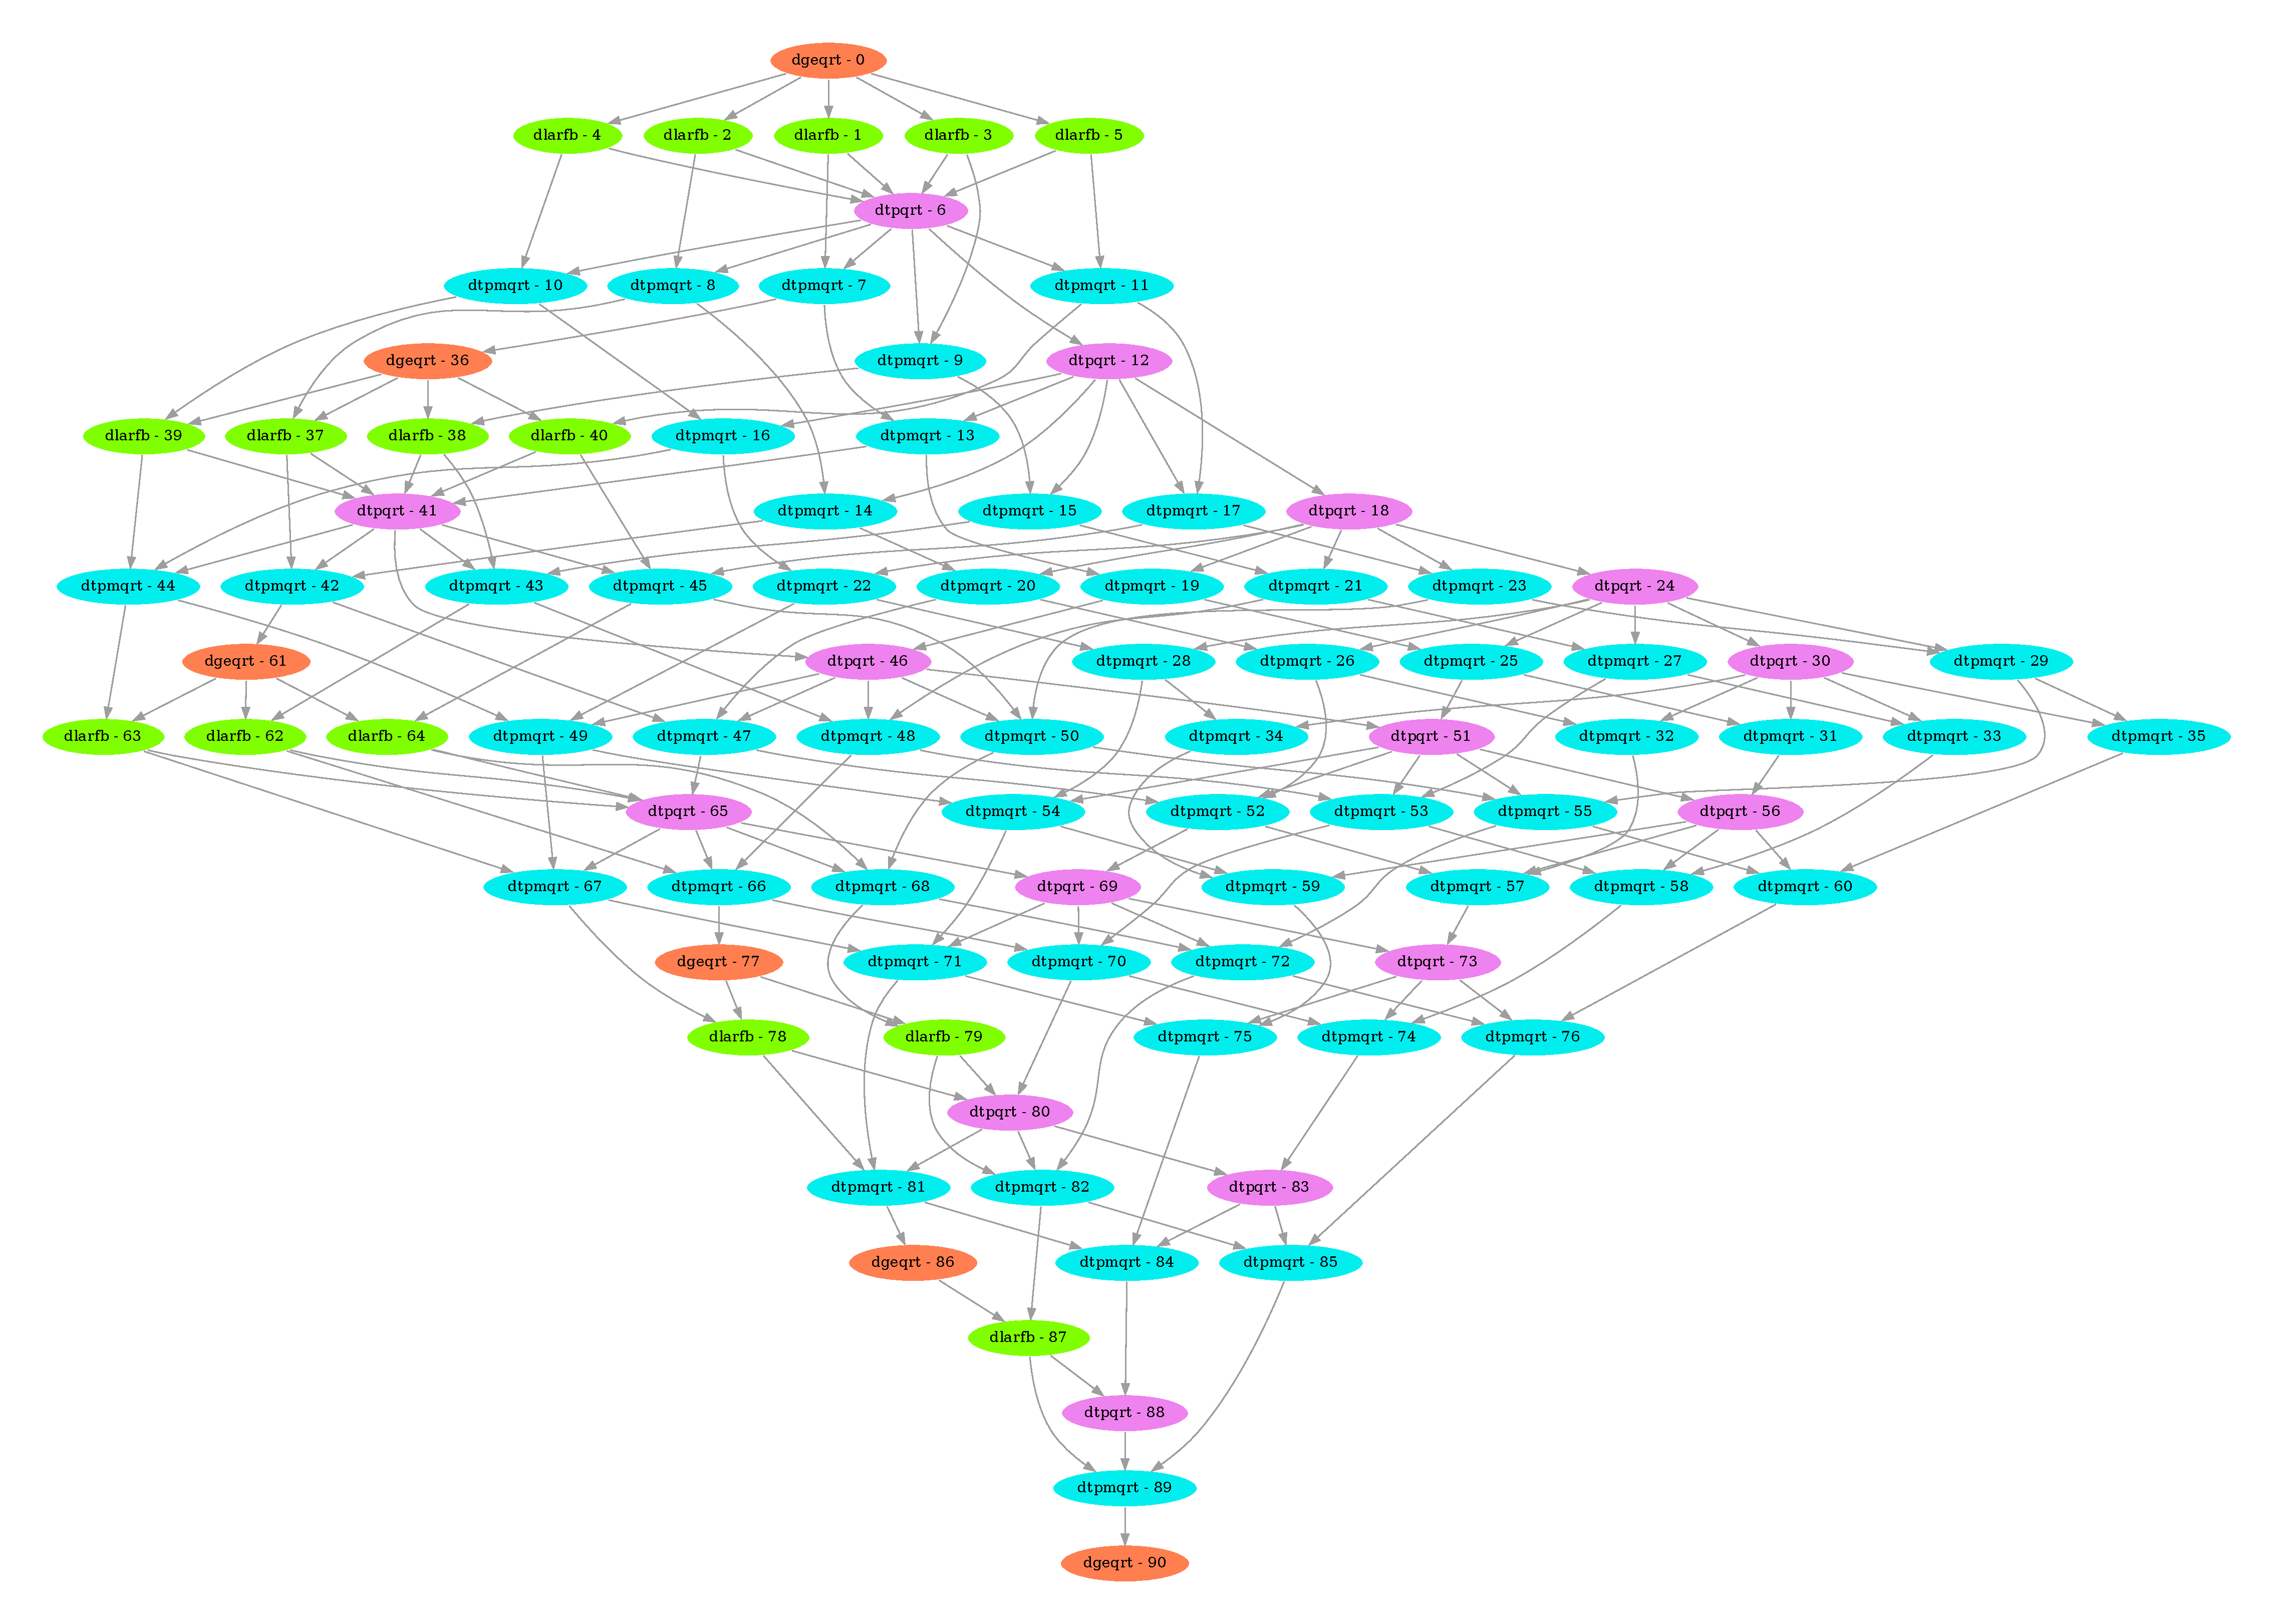
\includegraphics[width=1.05\textwidth]{dag1.pdf}
\end{center}
\end{column}

\begin{column}{0.5\columnwidth}
\alert{Programmer:} Define the tasks and its parameters.

\vspace{15px}
\alert{Runtime system:} Schedule tasks to the computational cores.
\end{column}
\end{columns}
\end{frame}



\begin{frame}[label={sec:orgb390aef}]{Task-based parallelism}
\begin{columns}
\begin{column}{0.4\columnwidth}
\small Can be viewed as a TDG (Task Dependency Graph)

\vspace{15px}
\end{column}

\begin{column}{0.6\columnwidth}
\begin{center}
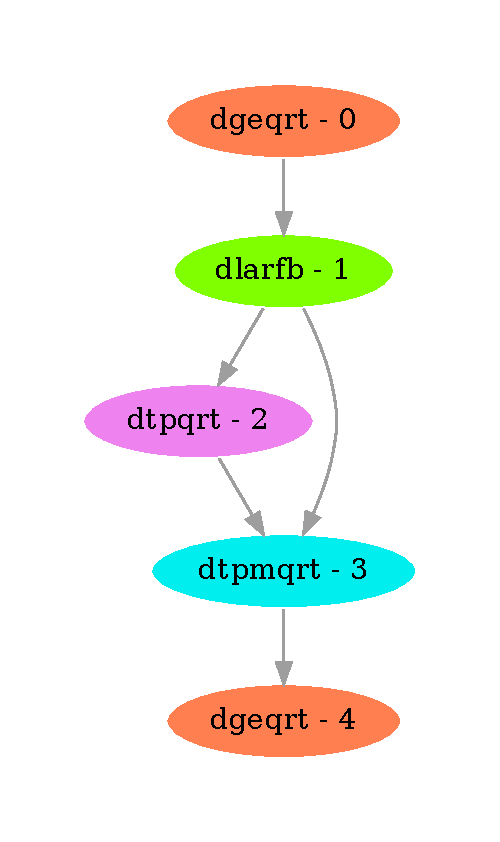
\includegraphics[width=0.4\textwidth]{dag-p.pdf}
\end{center}
\end{column}
\end{columns}
\end{frame}



\begin{frame}[label={sec:orgc6bef4a}]{OpenMP}
\begin{columns}
\begin{column}{0.6\columnwidth}
\begin{itemize}
\item Shared-memory multiprocessing programming interface.
\end{itemize}
\vspace{10px}
\begin{itemize}
\item Since 3.0 supports tasks.
\end{itemize}
\vspace{10px}
\begin{itemize}
\item New features for tasks with newer versions.
\end{itemize}
\end{column}



\begin{column}{0.4\columnwidth}
\begin{center}

\includegraphics[width=.9\linewidth]{imgs/openmp.png}
\end{center}
\end{column}
\end{columns}
\end{frame}


\begin{frame}[label={sec:orgb568cd6}]{OpenMP}
\begin{center}
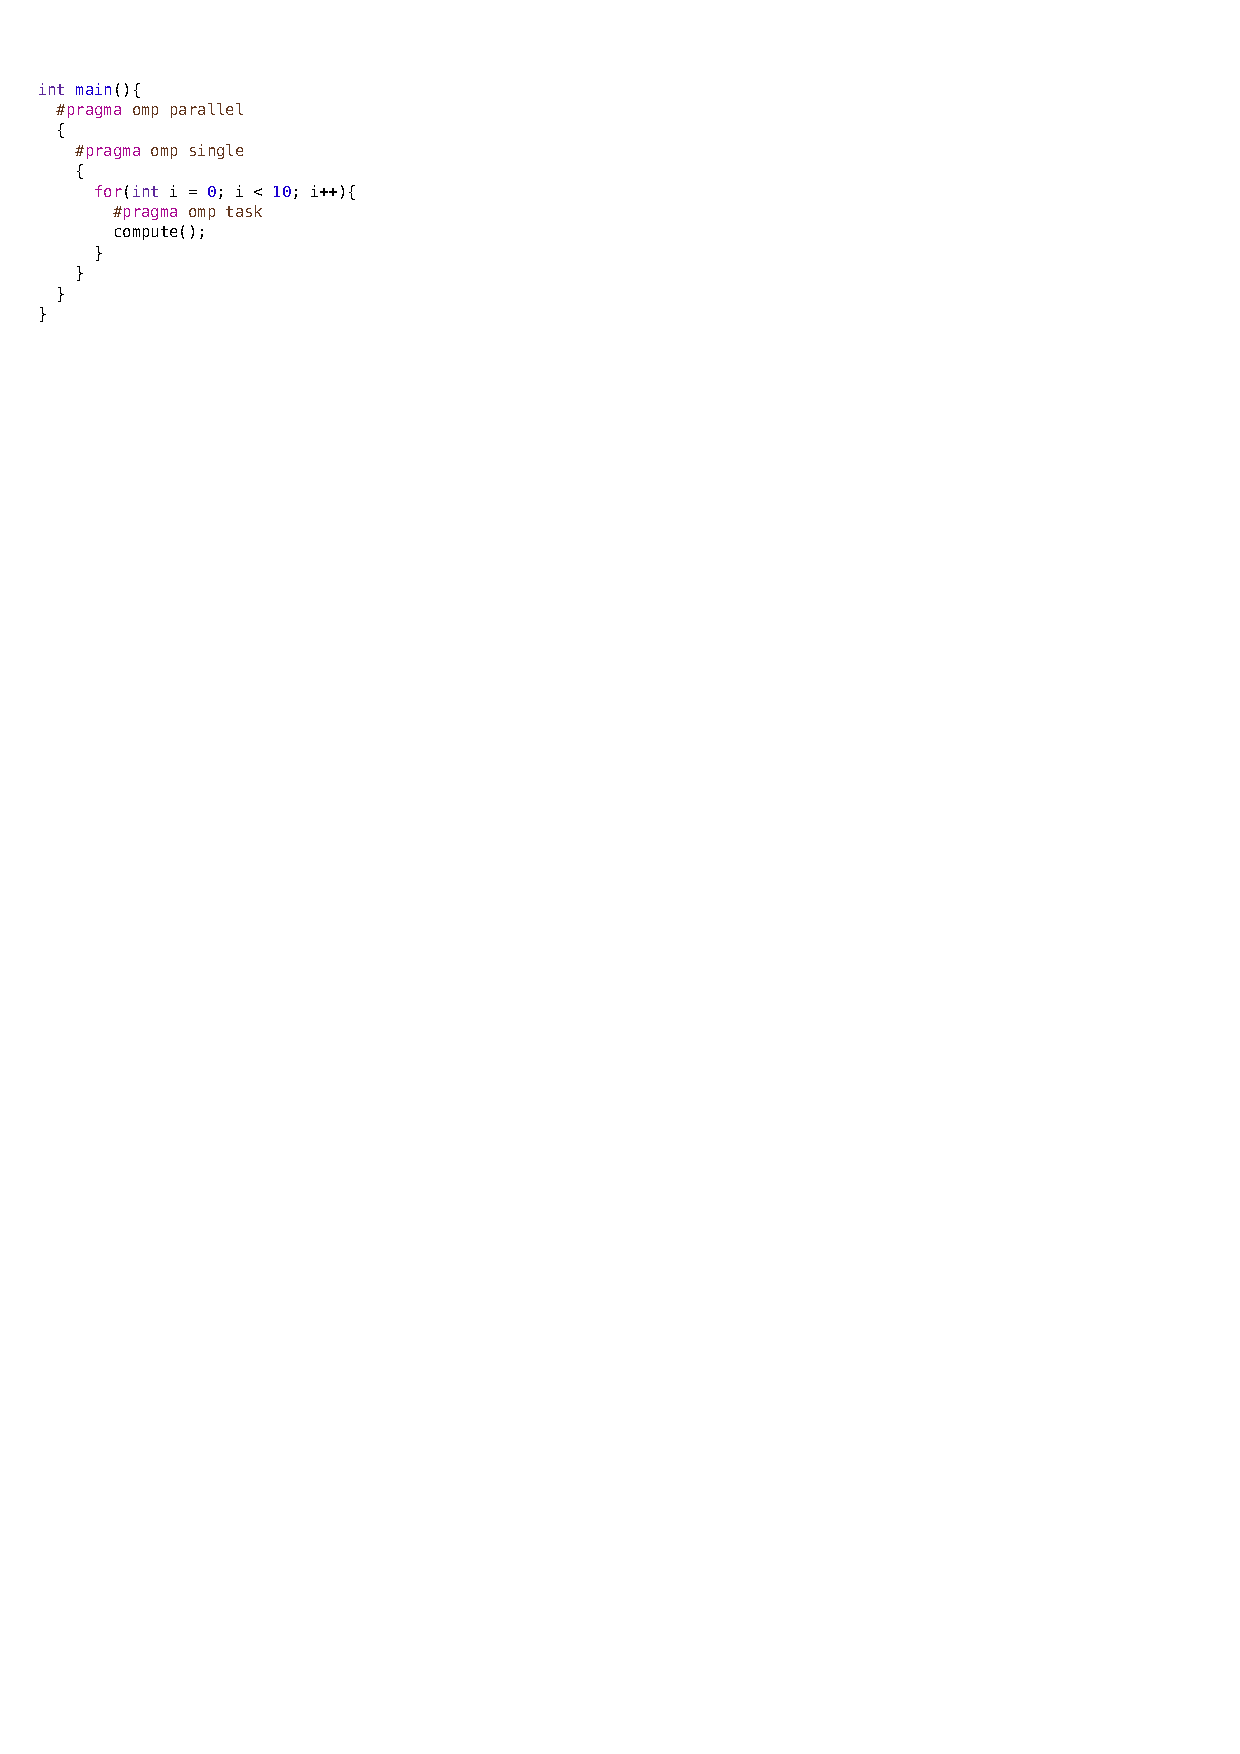
\includegraphics[width=0.6\textwidth]{imgs/tasks.pdf}
\end{center}
\end{frame}


\begin{frame}[label={sec:orge7ccbb4}]{Dynamic scheduling}
\begin{itemize}
\item Application behavior is not simple to understand.
\end{itemize}
\hfill \pause
\begin{itemize}
\item Need for tracing tools capable of capture tasks life cycle.
\end{itemize}
\end{frame}



\section{\small \color{mblack} Intrusiveness and Scalability of \color{R} OMPT-Based Tracing Tools  \color{mblack} for Task-based OpenMP Applications}
\label{sec:orgbdda08c}

\begin{frame}[label={sec:org740c34b}]{OMPT (OpenMP Tools)}
\begin{columns}
\begin{column}{0.5\columnwidth}
Introduced in OpenMP 5.

\vspace{10px}
User-defined callbacks when OpenMP events occurs.
\end{column}

\begin{column}{0.5\columnwidth}
\begin{center}
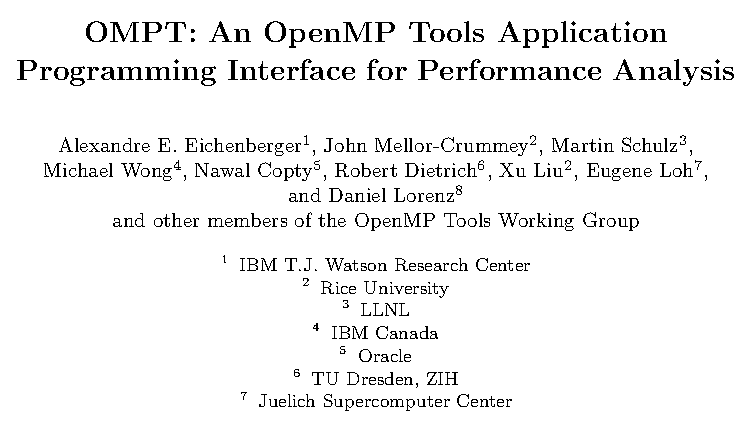
\includegraphics[width=.9\linewidth]{imgs/OMPT.pdf}
\end{center}
\end{column}
\end{columns}
\end{frame}

\begin{frame}[label={sec:orgcf88b43}]{Tracing}
\begin{itemize}
\item Additional code to trace application behavior.
\end{itemize}
\pause
\begin{itemize}
\item Changes the application environment and \alert{introduce overhead.}
\end{itemize}
\end{frame}

\begin{frame}[label={sec:orgd9fa81e}]{Tracing Tools}
\begin{columns}
\begin{column}{0.5\columnwidth}
\begin{block}{Our tools}
\begin{itemize}
\item Void
\item Printf
\item OOT
\end{itemize}
\end{block}
\end{column}


\begin{column}{0.5\columnwidth}
\begin{block}{Popular tools}
\begin{itemize}
\item Score-P
\item TiKKi
\item Extrae
\end{itemize}
\end{block}
\end{column}
\end{columns}
\end{frame}


\begin{frame}[label={sec:org735d5a9}]{Void}
\begin{center}
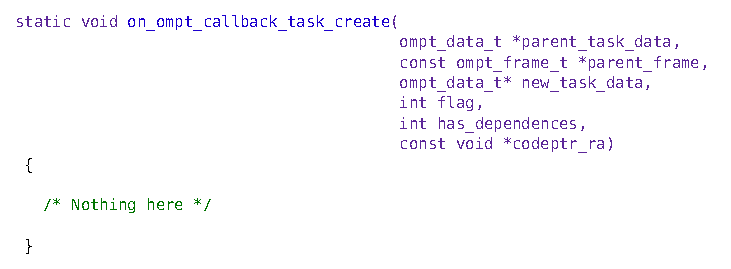
\includegraphics[width=.9\linewidth]{imgs/void.pdf}
\end{center}
\end{frame}

\begin{frame}[label={sec:org092be58}]{Printf}
\begin{center}
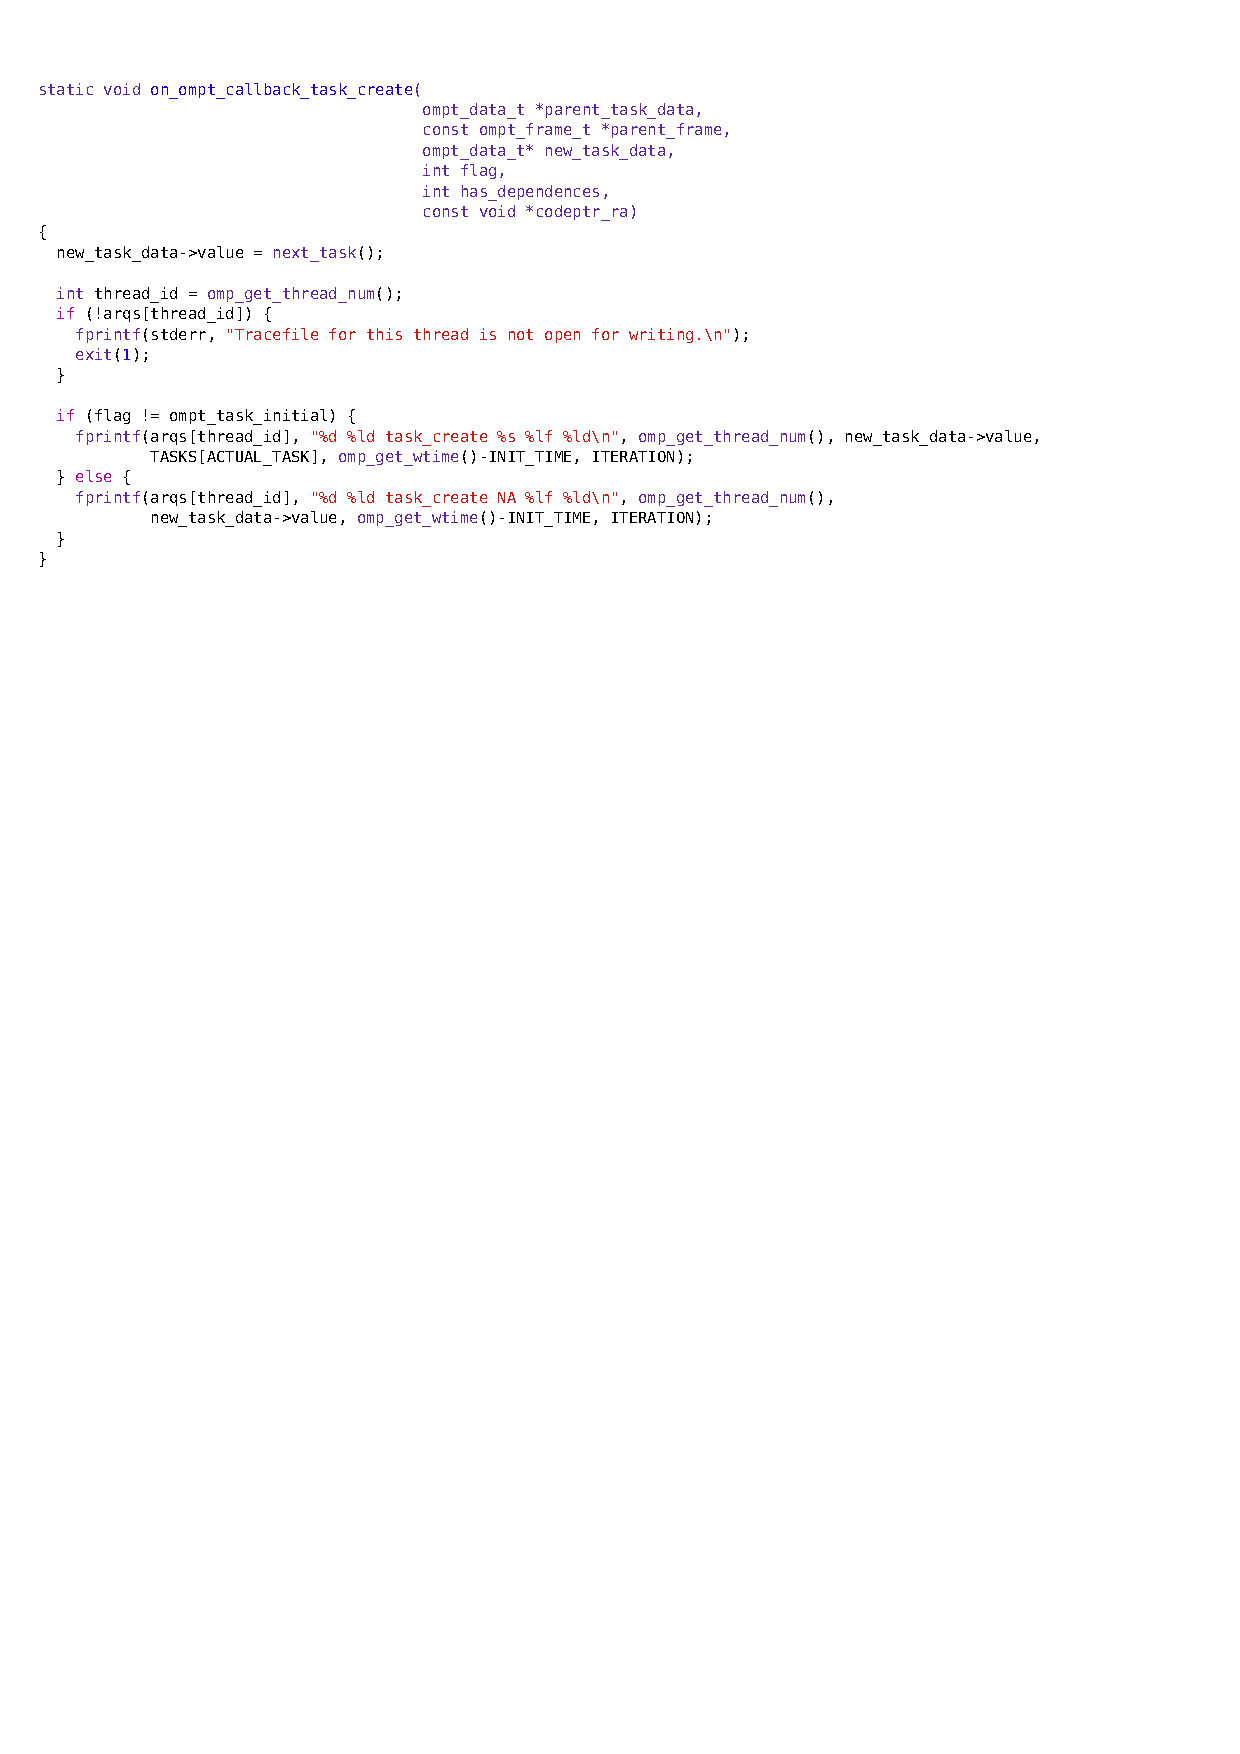
\includegraphics[width=.9\linewidth]{imgs/printf.pdf}
\end{center}
\end{frame}

\begin{frame}[label={sec:orgbf2d278}]{OOT}
\begin{center}
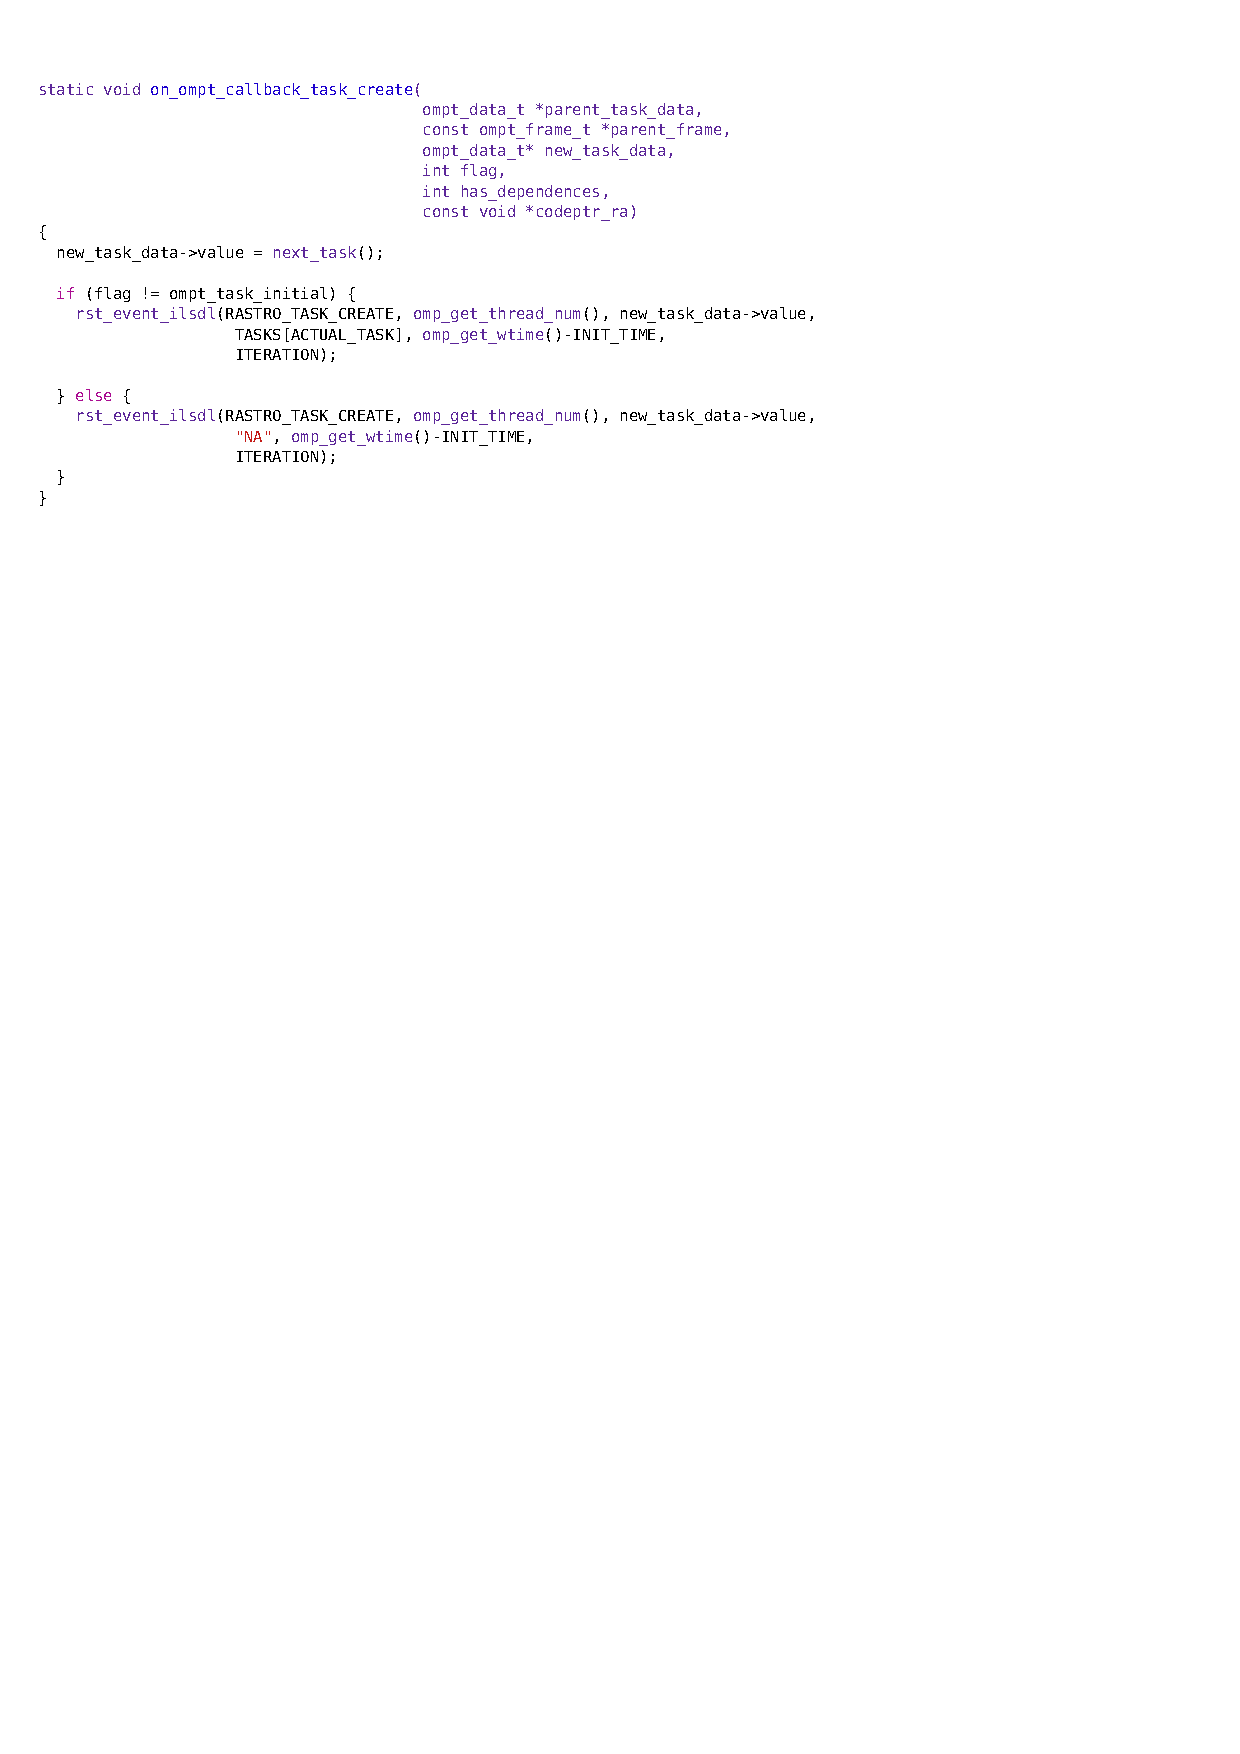
\includegraphics[width=.9\linewidth]{imgs/oot.pdf}
\end{center}
\end{frame}

\section{\small \color{R} Intrusiveness and Scalability \color{mblack} of OMPT-Based Tracing Tools for Task-based OpenMP Applications}
\label{sec:orgdbbfa8b}

\section{Methodology}
\label{sec:orgebbbec7}
\begin{frame}[label={sec:org18b06f9}]{Benchmark}
\begin{columns}
\begin{column}{0.6\columnwidth}
\begin{itemize}
\item QR Factorization
\end{itemize}

\vspace{10px}
\begin{itemize}
\item Gauss-Seidel
\end{itemize}
\vspace{10px}
\begin{itemize}
\item Cholesky Factorization
\end{itemize}
\end{column}


\begin{column}{0.4\columnwidth}
\end{column}
\end{columns}
\end{frame}

\begin{frame}[label={sec:org3168c3c}]{Application parameters}
\footnotesize
\begin{center}
\begin{tabular}{llll}
\toprule
\alert{Application} & \alert{Problem} & \alert{Block} & \alert{Tasks Created}\\
\midrule
QR factorization & 2048 & 64, 128, 192, 258 & 11440, 1496, 385, 204\\
Cholesky factorization & 2000 & 50, 80, 100, 200 & 11480, 2925, 1540, 220\\
Gauss-Seidel method & 10000 & 250, 500, 1000, 2000 & 16000, 4000, 1000, 250\\
\bottomrule
\end{tabular}
\end{center}
\end{frame}

\begin{frame}[label={sec:org6d5c5ce}]{Hardware configuration}
\footnotesize
\begin{center}
\begin{tabular}{lll}
\toprule
\alert{Nome} & \alert{CPU} & \alert{RAM}\\
\midrule
Cei & 2 x Intel(R) Xeon(R) Silver 4116, 2.10 GHz, 48 ths, 24 cores & 96 GB DDR4\\
Hype & 2 x Intel(R) Xeon(R) E5-2650 v3, 2.30 GHz, 40 ths, 20 cores & 128 GB DDR4\\
Draco & 2 x Intel(R) Xeon(R) E5-2640 v2, 2.00 GHz, 32 ths, 16 cores & 64 GB DDR3\\
\bottomrule
\end{tabular}
\end{center}
\end{frame}

\begin{frame}[label={sec:orgbcdeaee}]{Experiments}
\begin{itemize}
\item Full factorial (application, block, \# threads, etc\ldots{})
\end{itemize}
\hfill \pause
\begin{itemize}
\item 10 executions for each combination
\end{itemize}
\hfill \pause
\begin{itemize}
\item Metric: Intrusion time (overhead).
\end{itemize}
\end{frame}


\section{Results}
\label{sec:orgaf6ff8f}

\begin{frame}[label={sec:org9b06a9b}]{Intrusion overview (QR)}
\begin{center}
\includegraphics[width=.9\linewidth]{/tmp/babel-AjemSq/figurex4IqYG.pdf}
\end{center}
\end{frame}

\begin{frame}[label={sec:org9ec5f57}]{Intrusion overview (QR)}
\begin{center}
\includegraphics[width=.9\linewidth]{/tmp/babel-AjemSq/figure7OE8ZS.pdf}
\end{center}
\end{frame}

\begin{frame}[label={sec:org028bc01}]{Intrusion overview (QR)}
\begin{center}
\includegraphics[width=.9\linewidth]{/tmp/babel-AjemSq/figureA38rB1.pdf}
\end{center}
\end{frame}




\begin{frame}[label={sec:org305d133}]{Intrusion overview (QR)}
\begin{center}
\includegraphics[width=.9\linewidth]{/tmp/babel-AjemSq/figureFxkpoO.pdf}
\end{center}
\end{frame}

\begin{frame}[label={sec:org084715f}]{Intrusion overview (QR)}
\begin{center}
\includegraphics[width=.9\linewidth]{/tmp/babel-AjemSq/figureLTiRnd.pdf}
\end{center}
\end{frame}

\begin{frame}[label={sec:org2fc8415}]{Scalability: Void}
\begin{center}
\includegraphics[width=.9\linewidth]{/tmp/babel-AjemSq/figurei5Hoou.pdf}
\end{center}
\end{frame}

\begin{frame}[label={sec:org839c2d1}]{Scalability: Printf}
\begin{center}
\includegraphics[width=.9\linewidth]{/tmp/babel-AjemSq/figurelVjYai.pdf}
\end{center}
\end{frame}

\begin{frame}[label={sec:org55fcab2}]{Scalability: OOT}
\begin{center}
\includegraphics[width=.9\linewidth]{/tmp/babel-AjemSq/figureoZLN4R.pdf}
\end{center}
\end{frame}

\begin{frame}[label={sec:orgd4839cc}]{Scalability: Score-P}
\begin{center}
\includegraphics[width=.9\linewidth]{/tmp/babel-AjemSq/figurezdDuXY.pdf}
\end{center}
\end{frame}

\begin{frame}[label={sec:org70be40e}]{Scalability: TiKKi}
\begin{center}
\includegraphics[width=.9\linewidth]{/tmp/babel-AjemSq/figureME9PhY.pdf}
\end{center}
\end{frame}

\begin{frame}[label={sec:org1397c7a}]{Scalability: Extrae}
\begin{center}
\includegraphics[width=.9\linewidth]{/tmp/babel-AjemSq/figure7KlW86.pdf}
\end{center}
\end{frame}


\section{Conclusion}
\label{sec:org30edac0}
\begin{frame}[label={sec:org51d7114}]{Conclusions}
\begin{itemize}
\item The OMPT interface has a low intrusion by itself \alert{(Void)}.
\end{itemize}
\pause
\begin{itemize}
\item The choose of the tracer tool can impact the performance.
\end{itemize}
\pause
\begin{itemize}
\item Tracing tool choice is crucial depending on the expected result.
\end{itemize}
\end{frame}


\begin{frame}[label={sec:org82cd5f7}]{}
\begin{columns}
\begin{column}{0.6\columnwidth}
\begin{block}{\Huge \alert{Questions?}}
\vspace{40px}
Contact: rayan.raddatz@inf.ufrgs.br


\includegraphics[width=0.05\paperwidth]{./imgs/fundo_amanha.jpeg}
\includegraphics[width=0.1\paperwidth]{~/logos/CNPq.jpg}
\includegraphics[width=0.1\paperwidth]{~/logos/UFRGS.png}
\includegraphics[width=0.1\paperwidth]{~/logos/INF.png}
\end{block}
\end{column}



\begin{column}{0.4\columnwidth}

\includegraphics[width=0.3\paperwidth]{./imgs/companion.pdf}
\end{column}
\end{columns}
\end{frame}
\end{document}